\documentclass[border=4pt]{standalone}
\usepackage{tikz}
\usetikzlibrary{arrows.meta, positioning}

\begin{document}
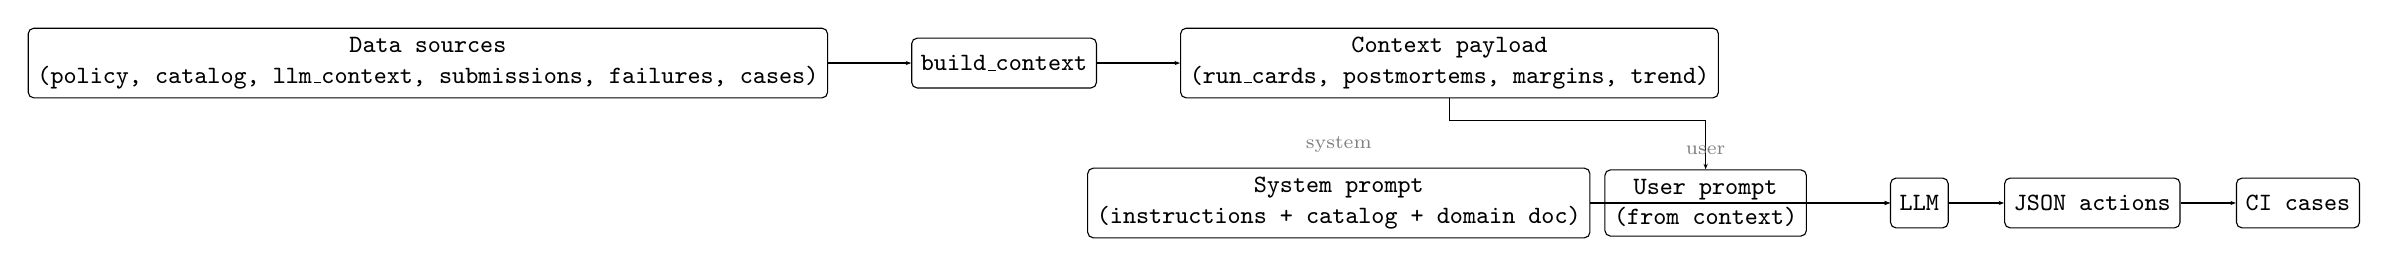
\begin{tikzpicture}[
  node distance=0.5em,
  box/.style={rectangle, draw, rounded corners=2pt, minimum height=1.8em, font=\small\tt},
  arr/.style={-{Stealth[length=2pt]}}
  ]
  \node[box, align=center] (src) {Data sources\\(policy, catalog, llm\_context, submissions, failures, cases)};
  \node[box, right=3em of src] (build) {build\_context};
  \node[box, align=center, right=3em of build] (ctx) {Context payload\\(run\_cards, postmortems, margins, trend)};
  \node[box, align=center, below=2.5em of ctx, xshift=-4em] (sys) {System prompt\\(instructions + catalog + domain doc)};
  \node[box, align=center, right=0.5em of sys] (usr) {User prompt\\(from context)};
  \node[box, right=3em of usr] (llm) {LLM};
  \node[box, right=2em of llm] (act) {JSON actions};
  \node[box, right=2em of act] (out) {CI cases};

  \draw[arr] (src) -- (build);
  \draw[arr] (build) -- (ctx);
  \draw[arr] (ctx.south) -- ++(0,-0.8em) -| (usr.north);
  \draw[arr] (sys) -- (llm);
  \draw[arr] (usr) -- (llm);
  \draw[arr] (llm) -- (act);
  \draw[arr] (act) -- (out);

  \node[font=\scriptsize, gray, above=0.2em of sys] {system};
  \node[font=\scriptsize, gray, above=0.2em of usr] {user};
\end{tikzpicture}
\end{document}
